% !TEX program = lualatex
% ECON 201, Midterm 1 study guide, in workbook form (Div chose this over an
% ECON 340-style topic list on 2026-10-06).
% Page 1: exam facts and how to study. Then one page per topic with the same parts: "Can
% you?" retrieval prompts the student rates themselves on, one worked example
% in exam format, and a twin problem with changed numbers and answers only;
% no working space on the sheet (Div, 2026-10-06). The design follows the evidence on
% retrieval practice, worked-example pairs, spacing, and self-assessment.
% Examples use their own firms and numbers, never the lectures'. Surplus
% figures come from figures/make_midterm1.py, which also prints the numbers.
% Build from the course root:
%   latexmk -lualatex -cd exams/midterm1/midterm1-study-guide.tex && latexmk -c -cd exams/midterm1/midterm1-study-guide.tex
\DocumentMetadata{
  pdfstandard=UA-2,
  pdfversion=2.0,
  lang=en-US,
  tagging=on
}
\documentclass[11pt]{article}
% Shared preamble for the Midterm 1 materials (help sheet, study guide,
% practice exams, solutions). \input after \documentclass. Every document
% that uses it starts with \DocumentMetadata and compiles under LuaLaTeX.
\usepackage[letterpaper, margin=0.75in, top=0.55in, bottom=0.6in]{geometry}
\usepackage{fontspec}
\setmainfont{Fira Sans}
\usepackage{amsmath}
% Math in the same family as the text; without this the formulas are set
% in Computer Modern and look pasted in from another document.
\usepackage{unicode-math}
\setmathfont{Fira Math}
\usepackage{graphicx}
\usepackage{booktabs}
\usepackage{array}
\usepackage{multicol}
\usepackage{needspace}
\usepackage{xcolor}
\usepackage[most]{tcolorbox}
\definecolor{accent}{HTML}{BF5700}
\definecolor{accentdark}{HTML}{8F4100}
\definecolor{cream}{HTML}{FDF3EA}
\definecolor{muted}{HTML}{595A5B}
\definecolor{rule}{HTML}{D9D9D9}
\usepackage{titlesec}
\titleformat{\section}{\Large\bfseries\color{accent}}{}{0pt}{}
\titlespacing*{\section}{0pt}{0pt}{4pt}
\titleformat{\subsection}{\normalsize\bfseries\color{accentdark}}{}{0pt}{}
\titlespacing*{\subsection}{0pt}{9pt}{2pt}
% Running header for the help sheet, as on the 340 and 441 sheets.
\usepackage{fancyhdr}
\fancypagestyle{sheet}{%
  \fancyhf{}\renewcommand{\headrulewidth}{0.4pt}%
  \fancyhead[L]{\small ECON 201: Principles of Microeconomics}%
  \fancyhead[R]{\small Midterm 1 Help Sheet}%
  \fancyfoot[C]{\small\thepage}}
\usepackage{hyperref}
\hypersetup{hidelinks}
\setlength{\parindent}{0pt}
\setlength{\parskip}{3pt}
\setlength{\abovedisplayskip}{4pt}
\setlength{\belowdisplayskip}{4pt}
\setlength{\abovedisplayshortskip}{2pt}
\setlength{\belowdisplayshortskip}{4pt}
\setlength{\columnsep}{22pt}

% Compact lists.
\makeatletter
\def\@listi{\leftmargin\leftmargini \topsep 2pt \partopsep 0pt \parsep 0pt \itemsep 1pt}
\let\@listI\@listi
\def\@listii{\leftmargin\leftmarginii \labelwidth\leftmarginii
  \advance\labelwidth-\labelsep \topsep 1pt \parsep 0pt \itemsep 0pt}
\makeatother

% Document header: title at left, course at right, with a rule beneath.
\newcommand{\docheader}[2]{%
  {\LARGE\bfseries\color{accent}#1}\hfill{\large #2}\par
  \vspace{2pt}{\color{accent}\rule{\linewidth}{0.8pt}}\par\vspace{6pt}}

% Panels. Cream for examples and reference material, white with an orange
% frame for things the student fills in. Text on cream uses accentdark
% (7.7:1), since the brand orange falls below 4.5:1 there.
\newtcolorbox{panel}[1]{colback=cream, colframe=accent, boxrule=0.6pt, arc=2pt,
  left=7pt, right=7pt, top=4pt, bottom=5pt, title=#1, fonttitle=\bfseries,
  coltitle=white, colbacktitle=accent, toptitle=2pt, bottomtitle=2pt,
  before skip=6pt, after skip=6pt}
\newtcolorbox{workpanel}[1]{colback=white, colframe=accent, boxrule=0.6pt, arc=2pt,
  left=7pt, right=7pt, top=4pt, bottom=5pt, title=#1, fonttitle=\bfseries,
  coltitle=white, colbacktitle=accent, toptitle=2pt, bottomtitle=2pt,
  before skip=6pt, after skip=6pt}
\newtcolorbox{notepanel}[1]{colback=white, colframe=muted, boxrule=0.5pt, arc=2pt,
  left=7pt, right=7pt, top=3pt, bottom=4pt, title=#1, fonttitle=\bfseries,
  coltitle=white, colbacktitle=muted, toptitle=1pt, bottomtitle=1pt,
  before skip=6pt, after skip=6pt}

% Pointers back to the course materials.
\newcommand{\where}[1]{{\color{muted}\small #1}}
% An empty box to tick by hand.
\newcommand{\tick}{{\large$\mdlgwhtsquare$}}
% Step label inside a worked example.
% Help sheet rows: the formula, then what its symbols mean. The argument
% is the width of the formula column; both cells are vertically centred so
% a note sits level with a tall fraction.
\newenvironment{formulas}[1]
  {\begin{tabular}{@{}>{\raggedright\arraybackslash$\displaystyle}m{#1}<{$}@{\hspace{10pt}}>{\small\color{muted}\raggedright\arraybackslash}m{\dimexpr\linewidth-#1-10pt\relax}@{}}}
  {\end{tabular}\par\vspace{3pt}}
\newcommand{\frow}{\\[5pt]}
% One formula on its own line, left-aligned, for the help sheet.
\newlength{\flskip}\setlength{\flskip}{5pt}
\newcommand{\fl}[1]{\par\noindent\hspace*{1em}$\displaystyle #1$\par\vspace{\flskip}}
% Exam pieces. \pts marks a part's points; \work leaves ruled space on an
% exam and nothing in its solutions; \sol prints only in the solutions.
\newif\ifsolutions
\def\ptsone{1}
\DeclareRobustCommand{\pts}[1]{{\def\ptsarg{#1}\color{muted}\small[#1~\ifx\ptsarg\ptsone pt\else pts\fi]}}
\pdfstringdefDisableCommands{\def\pts#1{}}
% A part of a problem: label and points, with air above it.
% A hint or aside under a part, in the muted colour.
\newcommand{\fnote}[1]{\par\vspace{2pt}{\small\color{muted}#1}\par}
% A physical sheet of the exam: starts on an odd page (a blank page is
% inserted if needed, so sheets can be separated and graded by different
% people) and carries a name and CWID line on its front.
% The CWID is nine boxes, one digit each, as on the scanned exam.
\newcommand{\cwidbox}{\fbox{\rule{0pt}{7mm}\hspace{5.5mm}}\hspace{0.6mm}}
\newcommand{\cwidboxes}{{\setlength{\fboxsep}{0pt}\setlength{\fboxrule}{0.5pt}%
  \cwidbox\cwidbox\cwidbox\cwidbox\cwidbox\cwidbox\cwidbox\cwidbox\cwidbox}}
\newcommand{\sheet}[1]{\clearpage\ifodd\value{page}\else\mbox{}\thispagestyle{empty}\clearpage\fi
  \noindent Name: \rule{7.5cm}{0.4pt}\par\vspace{8pt}
  \noindent CWID:\enspace\raisebox{-2.4mm}{\cwidboxes}\enspace{\small\color{muted}One digit per box.}\par\vspace{5pt}
  \noindent{\small\color{muted}#1}\par\vspace{6pt}}
% Multiple choice laid out like the scanned exam: the question and its
% options at left, a row of answer bubbles at right (exam copy only). The
% bubble is Fira Math's large circle; Fira Sans has none.
\newfontfamily\bubblefont{Fira Math}
\newcommand{\bubble}[1]{\shortstack{{\bubblefont\large ◯}\\[-1pt]{\scriptsize\color{muted}#1}}}
\newcommand{\mcopt}[2]{\par\noindent\hangindent=1.8em\hangafter=1\makebox[1.8em][l]{(#1)}#2}
\newcommand{\mcq}[5]{\item\ifsolutions\begin{minipage}[t]{\linewidth}\else\begin{minipage}[t]{0.74\linewidth}\fi
  #1\par\vspace{3pt}\mcopt{A}{#2}\mcopt{B}{#3}\mcopt{C}{#4}\mcopt{D}{#5}\end{minipage}%
  \ifsolutions\else\hfill\begin{minipage}[t]{0.22\linewidth}\raggedleft
  \bubble{A}\hspace{5pt}\bubble{B}\hspace{5pt}\bubble{C}\hspace{5pt}\bubble{D}\end{minipage}\fi\par}
\newcommand{\qpart}[2]{\par\vspace{10pt}\noindent(#1) \pts{#2} }
% A numbered short-answer question: number and points, with more air above
% it than a part.
\newcommand{\sa}[2]{\par\vspace{14pt}\noindent\textbf{#1.} \pts{#2} }
\newcount\answerlinecount
\newcommand{\answerlines}[1]{%
  \par\vspace{1pt}\answerlinecount=#1
  \loop\ifnum\answerlinecount>0
    \rule{\linewidth}{0.3pt}\par\vspace{6pt}%
    \advance\answerlinecount by -1
  \repeat
  \vspace{-6pt}}
% Blank working space on an exam, about #1 lines of handwriting; nothing in
% the solutions. Ruled lines get in the way of fractions and arithmetic.
\newlength{\workline}\setlength{\workline}{18pt}
\newcommand{\work}[1]{\ifsolutions\else\par\vspace{#1\workline}\fi}
\newcommand{\sol}[1]{\ifsolutions\par\vspace{1pt}{\color{accentdark}\textbf{Solution.} #1}\par\fi}
\newcommand{\blankrow}{\rule{0pt}{1.9em}}
% Percentage change, as in the slides.
\newcommand{\pc}{\%\,\Delta}
\newcommand{\step}[1]{\textbf{\color{accentdark}#1}\enspace}

\hypersetup{pdftitle={ECON 201 Midterm 1 Study Guide}, pdfauthor={Div Bhagia}, colorlinks=true, linkcolor=accent}
\pagestyle{plain}
% Topic pages carry the topic's name in a running header (Div, 2026-10-06).
\newcommand{\topicname}{}
\fancypagestyle{topic}{%
  \fancyhf{}\renewcommand{\headrulewidth}{0pt}%
  \fancyhead[L]{\small\color{muted}Midterm 1 Study Guide}%
  \fancyhead[R]{\small\color{muted}\topicname}%
  \fancyfoot[C]{\small\thepage}}

\setlength{\parskip}{3pt}
\geometry{margin=0.7in, top=0.7in, bottom=0.5in, headheight=14pt, headsep=10pt}
\makeatletter
\def\@listi{\leftmargin\leftmargini \topsep 2pt \partopsep 0pt \parsep 0pt \itemsep 2pt}
\let\@listI\@listi
\makeatother
% Blocks are set by typography, not boxes: a small accent heading over a
% thin rule, then the content in one column.
% Topic titles one point larger than the shared style's \Large (17.28pt).
\titleformat{\section}{\fontsize{18.28}{22}\selectfont\bfseries\color{accent}}{}{0pt}{}
\newcommand{\block}[1]{\needspace{4\baselineskip}\par\vspace{6pt}\noindent{\fontsize{13}{16}\selectfont\bfseries\color{accent}#1}\par\vspace{-5pt}\noindent{\color{accent}\rule{\linewidth}{0.4pt}}\par\vspace{1pt}}
% Topic page header: title, lectures, and the one line of pointers.
% Each topic is two pages (the demand-and-costs topic is four; on the market
% power sheet Your Turn follows the worked example without a page break): a front with "Can you?" and the worked example,
% a back with "Your turn". Topics start on a new
% page, an odd one, so each topic is one physical sheet; page 2 holds the
% overview, so no page is blank (Div, 2026-10-06).
\newcommand{\topicpage}{\clearpage\ifodd\value{page}\else\mbox{}\thispagestyle{empty}\clearpage\fi}
\newcommand{\topic}[2]{\pagestyle{topic}\renewcommand{\topicname}{#1}\section{#1}\label{topic:#1}\vspace{-6pt}{\color{muted}#2.}\par}
% A lecture label inside a "Can you?" list that spans lectures, so each
% prompt points to the deck it comes from, in slide order.
\newcommand{\lec}[1]{\par\vspace{3pt}\noindent{\fontsize{11}{13.6}\selectfont\bfseries\color{accent}#1}\par\vspace{-2pt}}
% A "Can you?" prompt: one box, then the prompt.
\newcommand{\cy}[1]{\item[\tick] #1}
% Step label inside a worked example.
\renewcommand{\step}[1]{\par\vspace{1pt}\noindent\textbf{\textcolor{accent}{#1}}\enspace}
% A key word in running text (the names of the parts of a sheet), in the same style.
\newcommand{\kw}[1]{\textbf{\textcolor{accent}{#1}}}
% Answers to a twin problem.
\newcommand{\answers}[1]{\par\vspace{4pt}{\small\color{muted}\kw{Answers.} #1}\par}
% Table cells.
\newcolumntype{R}{>{\raggedleft\arraybackslash}p{1.6cm}}
\newcolumntype{Z}{>{\centering\arraybackslash}p{1.6cm}}
\newcolumntype{Y}{>{\centering\arraybackslash}p{1.2cm}}
\newcolumntype{W}{>{\centering\arraybackslash}p{1.45cm}}

\begin{document}

\docheader{Midterm 1 Study Guide}{ECON 201}

\block{Exam Logistics}
\begin{itemize}\setlength{\itemsep}{6pt}
\item Monday, October 12, in class, 65 minutes. Lectures 3 to 13.
\item The exam has three parts, weighted equally:
\par\vspace{4pt}
\begin{enumerate}\setlength{\itemsep}{2pt}
\item multiple-choice questions;
\item short-answer problems;
\item one long-form question.
\end{enumerate}
\vspace{5pt}Each part is its own sheet, printed front and back. The sheets are graded separately and matched by CWID, so \textbf{write your name and your CWID, one digit per box, at the top of every sheet}. The practice exam, posted with solutions on the course website, has the same layout.
\item Closed book, closed notes. Bring a basic calculator. You will be given the help sheet, which is posted on the course website.
\end{itemize}

\block{How to Prepare?}
For each topic, follow the structure of the guide:
\begin{enumerate}\setlength{\itemsep}{6pt}
\item Go over the slides for that topic.
\item Then close them and run the \kw{Can You?} list, answering each line out loud or on paper. Tick a line when you can do it without looking.
\item If you cannot answer a line, go back to the slides, the textbook sections, and the practice problems for that topic and review them. Do not move on until you can.
\item Read the \kw{Worked Example}, then turn the page and do \kw{Your Turn} on your own, without looking back. Check it against the answers at the back. If you got something wrong, find where in the worked example, and mark the topic to revisit.
\item If you feel confident at this point, move on to the next topic; otherwise do more problems on the worksheets and practice pages, and look at the textbook sections for clarity.
\end{enumerate}

Once you have been through every topic, take the practice exam, timed, with only the help sheet. Then grade it with the solutions and go back to the topics where you lost points.

If you get stuck at any point or need help with the material, feel free to send me an email.


% =====================================================================
\newpage
\section{Overview}
Each topic has its own sheet; click a title to jump to it. The front holds the \kw{Can You?} list and a worked example, the back a problem for you. Answers to the problems are on the last page.

\vspace{6pt}
\begin{center}
\renewcommand{\arraystretch}{1.3}
\begin{tabular}{@{}>{\raggedright\arraybackslash}p{\dimexpr\linewidth-6.5cm\relax}>{\raggedright\arraybackslash}p{3.5cm}>{\centering\arraybackslash}p{2cm}@{}}
\toprule
Topic & Lectures & Page \\
\midrule
\hyperref[topic:Opportunity Cost and Economic Rent]{Opportunity Cost and Economic Rent} & 3 & \pageref{topic:Opportunity Cost and Economic Rent} \\
\hyperref[topic:Specialization and Comparative Advantage]{Specialization and Comparative Advantage} & 4 & \pageref{topic:Specialization and Comparative Advantage} \\
\hyperref[topic:Costs, Demand, and the Profit-Maximizing Choice]{Costs, Demand, and the Profit-Maximizing Choice}* & 5, 6, and 9 & \pageref{topic:Costs, Demand, and the Profit-Maximizing Choice} \\
\hyperref[topic:Elasticity]{Elasticity} & 7 and 8 & \pageref{topic:Elasticity} \\
\hyperref[topic:Surplus and Efficiency]{Surplus and Efficiency} & 10 and 11 & \pageref{topic:Surplus and Efficiency} \\
\hyperref[topic:Market Power and Competition]{Market Power and Competition} & 12 and 13 & \pageref{topic:Market Power and Competition} \\
\hyperref[answers]{Answers to Your Turn} & & \pageref{answers} \\
\bottomrule
\end{tabular}
\end{center}
* This topic combines three lectures, so it runs slightly longer, two sheets instead of one. Allocate your time accordingly.

% =====================================================================
\topicpage
\topic{Opportunity Cost and Economic Rent}{Lecture 3}

\block{Can You? After Going Over the Slides, Check What Stuck}
\begin{itemize}
\cy{Say how to put a number on a benefit or a cost that does not have a price.}
\cy{Define opportunity cost in one sentence that uses the words ``outside option''.}
\cy{State the decision rule two ways: with net benefit and opportunity cost, and with benefit and economic cost.}
\cy{Define economic rent, and say what positive and zero rent mean for the decision.}
\cy{Explain why a shop with an accounting profit can be an economic loss.}
\end{itemize}

\block{Worked Example: Should Rafael Go to the Festival?}
Rafael can spend Saturday at a music festival or work a catering shift. The festival day is worth \$160 to him and costs \$90 in tickets and food. The shift pays \$100, and the least he would accept to give up a free Saturday for it is \$70.

\step{Net Benefit of Each Option.} Two of these numbers have no price tag. For the festival the cost is priced and Rafael judges the benefit: \$160 is the most he would pay for the day, his willingness to pay. For the shift the benefit is priced and he judges the cost: \$70 is the least he would accept to give up a free Saturday.

\begin{center}
\vspace{2pt}
\begin{tabular}{@{}lRR@{}}
\toprule
 & Festival & Shift \\
\midrule
Benefit & 160 & 100 \\
Direct cost & 90 & 70 \\
\midrule
Net benefit & 70 & 30 \\
\bottomrule
\end{tabular}
\vspace{2pt}
\end{center}

\step{Opportunity Cost.} The opportunity cost of the festival is the net benefit of its next best alternative, the shift: \$30.

\step{Decide.} Net benefit \$70 $>$ opportunity cost \$30, so Rafael goes.

\step{Economic Cost.} Direct cost plus opportunity cost: $90 + 30 = 120$. Benefit \$160 $>$ \$120, the same decision stated the other way.

\step{Economic Rent.} Net benefit minus opportunity cost: $70 - 30 = 40$. Positive, so the festival beats the shift.

\newpage
\block{Your Turn}
Priya can go to a concert or tutor for the evening. The concert is worth \$120 to her and costs \$50. Tutoring pays \$90, and the least she would accept to give up a free evening for it is \$45.

(a) Find the benefit, direct cost, and net benefit of each option.

(b) What is the opportunity cost of the concert?

(c) Should Priya go to the concert? Decide using net benefit and opportunity cost.

(d) What is the economic cost of the concert? Decide again using benefit and economic cost.

(e) What is the economic rent of the concert?


% =====================================================================
\topicpage
\topic{Specialization and Comparative Advantage}{Lecture 4}

\block{Can You? After Going Over the Slides, Check What Stuck}
\begin{itemize}
\cy{Say what a sunk cost is and why it should not affect a decision.}
\cy{Define absolute and comparative advantage in one sentence each.}
\cy{Given what two people can each make in an hour with the same resources, find each one's opportunity cost of one good in terms of the other, and use it to say who has the comparative advantage in which good.}
\cy{For the two people in the point above, find the range of prices at which both gain from trade, and say which end of the range favors whom.}
\cy{Explain why there are gains from trade even if one party has the absolute advantage in both goods.}
\end{itemize}

\block{Worked Example: Nia and Omar Make Lunch}
In an hour, Nia can make 12 salads or 4 sandwiches. Omar can make 2 salads or 4 sandwiches.

\step{Absolute Advantage.} Nia makes more salads and as many sandwiches, so she has the absolute advantage in salads and neither has one in sandwiches.

\step{Opportunity Costs.} Give up $\div$ get: an hour on sandwiches gives Nia 4 of them at the cost of 12 salads, so one sandwich costs her 3 salads.

\begin{center}
\vspace{2pt}
\begin{tabular}{@{}lll@{}}
\toprule
Cost of one & sandwich & salad \\
\midrule
Nia & $12/4 = 3$ salads & $4/12 = \tfrac{1}{3}$ sandwich \\
Omar & $2/4 = \tfrac{1}{2}$ salad & $4/2 = 2$ sandwiches \\
\bottomrule
\end{tabular}
\vspace{2pt}
\end{center}

\step{Comparative Advantage.} Whoever gives up less has it. A sandwich costs Omar $\tfrac{1}{2}$ salad and Nia 3, so Omar has the comparative advantage in sandwiches; a salad costs Nia $\tfrac{1}{3}$ sandwich and Omar 2, so Nia's is in salads. Nobody has it in both: a low cost of one good is a high cost of the other.

\step{Specialize.} On their own, say each spends $\tfrac{3}{4}$ of the hour on salads and $\tfrac{1}{4}$ on sandwiches. Nia makes $\tfrac{3}{4} \times 12 = 9$ salads and $\tfrac{1}{4} \times 4 = 1$ sandwich; Omar makes $\tfrac{3}{4} \times 2 = 1.5$ salads and $\tfrac{1}{4} \times 4 = 1$ sandwich. Together they make $9 + 1.5 = 10.5$ salads and $1 + 1 = 2$ sandwiches. Specialized, Nia on salads and Omar on sandwiches, they make 12 salads and 4 sandwiches, more of both.

\step{Trade.} Specializing only pays if they can trade, since each wants both goods. Say, Omar sells Nia 2 sandwiches for 2 salads. Nia ends with 10 salads and 2 sandwiches (was 9 and 1 when working alone); Omar with 2 salads and 2 sandwiches (was 1.5 and 1). Each has more of both.

\step{Prices That Work.} Omar sells a sandwich only above $\tfrac{1}{2}$ salad, its cost to him; Nia buys only below 3 salads, its cost to her. Any price between $\tfrac{1}{2}$ and 3 salads per sandwich works. Near $\tfrac{1}{2}$ favors Nia, near 3 favors Omar.

\newpage
\block{Your Turn}
In an hour, Ava can bake 8 cupcakes or 2 pies. Ben can bake 3 cupcakes or 3 pies.

(a) Who has the absolute advantage in each good?

(b) Find each person's opportunity cost of one pie and of one cupcake.

(c) Who has the comparative advantage in which good, and who should specialize in what?

(d) Ben sells Ava one pie for 2 cupcakes. Does each of them gain? Explain using the opportunity costs.

(e) Give the range of prices, in cupcakes per pie, at which both gain from trade.


% =====================================================================
\topicpage
\topic{Costs, Demand, and the Profit-Maximizing Choice}{Lectures 5, 6, and 9}

\block{Can You? After Going Over the Slides, Check What Stuck}
\lec{Lecture 5}
\begin{itemize}
\cy{Given a price $P$, a quantity $Q$, and a total cost function $C(Q)$, calculate revenue and profit, and, for a list of prices, pick the one with the highest profit.}
\cy{Explain the price-quantity trade-off a firm faces and why it cannot choose both. Say what the demand curve shows and what the law of demand is.}
\cy{Explain why a differentiated product gives a firm more control over its price.}
\end{itemize}
\lec{Lecture 6}
\begin{itemize}
\cy{Sort a firm's expenses into fixed and variable, and say why the answer depends on the time horizon (the short run and the long run).}
\cy{Explain why a factory the firm already owns is not free (the opportunity cost of capital).}
\cy{Explain in words what average cost and marginal cost are.}
\cy{Given a fixed cost and a cost per unit, write $C(Q) = F + cQ$, compute AC and MC at any $Q$, and explain why AC falls as $Q$ rises and stays above MC, and what happens with no fixed cost.}
\cy{Define increasing, decreasing, and constant returns to scale by what happens when a firm doubles all its inputs, and name them economies and diseconomies of scale.}
\cy{Give some reasons firms get big, and a reason they stop growing.}
\end{itemize}
\lec{Lecture 9}
\begin{itemize}
\cy{Say what willingness to pay (WTP) means and read a buyer's WTP off the demand curve, from its equation or its plot. (Also see slides 3 to 5 of lecture 7.)}
\cy{If you are given a demand curve as $Q = a - bP$, rearrange it to $P = a/b - Q/b$, and the other way around. Draw it with price on the vertical axis.}
\cy{Read off the demand curve the corresponding quantity for a given price, or the price for a given quantity, from its equation or its plot alone.}
\cy{Compute MR at a given quantity, and explain why MR is less than the price at any quantity.}
\cy{Know that the profit-maximizing quantity is where $\text{MR} = \text{MC}$ (you can see this directly from the plot, or from calculating MR at select quantities). Explain why profit is highest there.}
\cy{Explain why a higher fixed cost leaves the best price and quantity unchanged, and what decision it does affect.}
\end{itemize}

\block{Worked Example: A Juice Stand}
A juice stand's demand curve is $Q = 100 - 5P$. It pays \$50 a day for its spot, and each cup costs \$4 in fruit and ice.

\step{Costs.} The \$50 is fixed and the \$4 per cup is variable: $C(Q) = 50 + 4Q$. The cost of one more cup is $\text{MC} = \Delta C / \Delta Q = C(Q+1) - C(Q) = 4$ at every $Q$. The cost per cup is $\text{AC} = C(Q)/Q = (50 + 4Q)/Q = 4 + 50/Q$. It falls as the \$50 is spread over more cups (\$9 at $Q = 10$, \$6.50 at $Q = 20$) and always stays above the \$4 MC.

\step{Demand Curve.} $Q = 100 - 5P$: every \$1 rise in price sells 5 fewer cups; at $P = 0$ there are 100 buyers in the market, at $P = 20$ none. Rearranged, $5P = 100 - Q$, so $P = 20 - Q/5$. Both forms are the same curve: use whichever the question makes easier. Plot it with price on the vertical axis; in this form the slope is $\Delta P / \Delta Q = -1/5$.

\begin{center}
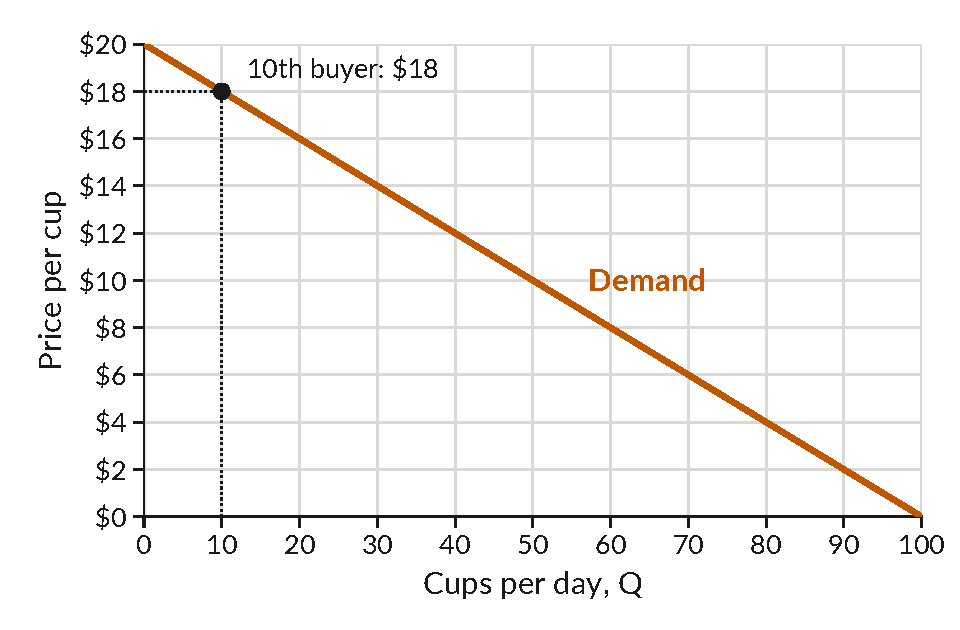
\includegraphics[width=0.55\linewidth, alt={The juice stand's demand curve, price per cup from 0 to 20 dollars on the vertical axis and cups per day from 0 to 100 on the horizontal axis. A straight line falls from 20 dollars at zero cups to zero at 100 cups. A marked point at 10 cups and 18 dollars, with dotted guides to both axes, is labelled 10th buyer: 18 dollars.}]{figures/juice.pdf}
\end{center}

\step{Willingness to Pay.} A buyer's willingness to pay (WTP) is the most they would pay for a cup. The height of the demand curve at any $Q$ is the WTP of the $Q$th buyer, so the 10th buyer's WTP is $20 - 10/5 = \$18$. Why: a buyer buys only if their WTP is at least the price. At \$18 ten cups sell, so ten buyers have a WTP of \$18 or more; at any price above \$18 fewer than ten do. So the 10th buyer's WTP is exactly \$18.

\step{Revenue, Cost, and Profit.} At $Q = 20$ the price is $P = 20 - 20/5 = 16$, so revenue is $R(20) = 16 \times 20 = 320$, cost is $C(20) = 50 + 4 \times 20 = 130$, average cost is $\text{AC} = 130/20 = 6.50$, and profit is $320 - 130 = 190$. The last four columns look one cup ahead. Selling a 21st cup needs the price $P(21) = 20 - 21/5 = 15.80$, so revenue becomes $R(21) = 15.80 \times 21 = 331.80$. The 21st cup adds $\text{MR} = R(21) - R(20) = 331.80 - 320 = 11.80$ to revenue and $\text{MC} = 4$ to cost. The table repeats this at other quantities.

\begin{center}
\vspace{2pt}
\setlength{\tabcolsep}{4pt}
\begin{tabular}{@{}WWWWWWWWWW@{}}
\toprule
$Q$ & $P$ & $R(Q)$ & $C(Q)$ & AC & Profit & $P(Q+1)$ & $R(Q+1)$ & MR & MC \\
\midrule
20 & 16 & 320 & 130 & 6.50 & 190 & 15.80 & 331.80 & 11.80 & 4 \\
30 & 14 & 420 & 170 & 5.67 & 250 & 13.80 & 427.80 & 7.80 & 4 \\
40 & 12 & 480 & 210 & 5.25 & 270 & 11.80 & 483.80 & 3.80 & 4 \\
50 & 10 & 500 & 250 & 5.00 & 250 & 9.80 & 499.80 & $-0.20$ & 4 \\
\bottomrule
\end{tabular}
\vspace{2pt}
\end{center}

\step{Marginal Revenue.} $\text{MR} = R(Q+1) - R(Q)$ is what one more cup adds to revenue, and it is less than the price of that cup. The 21st cup sells for \$15.80 but adds only \$11.80, because selling it means the other 20 cups now sell for 20 cents less each: $15.80 - 20 \times 0.20 = 11.80$. The same happens at every quantity, so in the table MR is always below $P(Q+1)$.

\step{The Profit-Maximizing Quantity and Price.} One more cup raises profit while $\text{MR} > \text{MC}$ and lowers it once $\text{MR} < \text{MC}$, so profit peaks where $\text{MR} = \text{MC}$. In the table, the 21st and 31st cups add \$11.80 and \$7.80 to revenue, more than their \$4 cost, so the stand should keep going. The 41st cup adds only \$3.80, less than \$4, so it should stop at 40; the 40th cup itself adds $R(40) - R(39) = 480 - 475.80 = 4.20$, still above MC. So $Q^* = 40$, and the demand curve gives $P^* = 20 - 40/5 = \$12$. Choosing $Q$ and choosing $P$ are the same decision, since the demand curve ties each price to one quantity. Profit is $480 - 210 = \$270$, the highest in the table.

\step{The Same Choice on a Plot.} Mark the table's MR values on the plot of the demand curve: they lie on a straight line, the MR line, which starts at the same point as demand and falls twice as steeply. It crosses the flat MC line at $Q = 40$, the point $E'$; straight up on the demand curve is $E$, at \$12.

\begin{center}
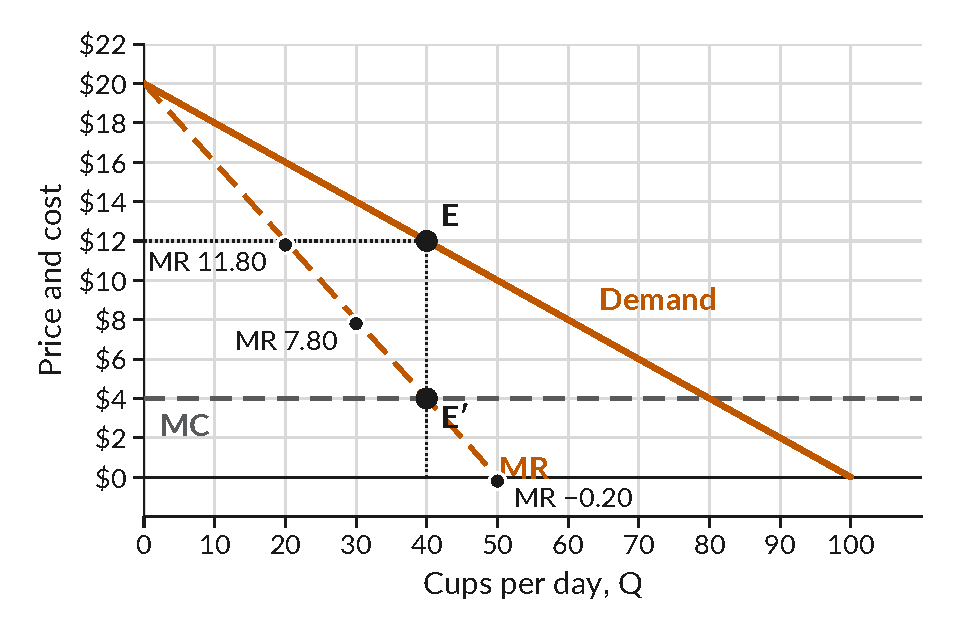
\includegraphics[width=0.75\linewidth, alt={Price and cost from minus 2 to 22 dollars on the vertical axis and cups per day from 0 to 110 on the horizontal. The demand curve falls in a straight line from 20 dollars at zero cups to zero at 100 cups. A dashed marginal revenue line falls twice as steeply from the same point, reaching zero at 50 cups, with the table's marginal revenue values marked as points at 20, 30, and 50 cups, labelled MR 11.80, MR 7.80, and MR minus 0.20. Marginal cost is a flat dashed line at 4 dollars. Marginal revenue meets marginal cost at 40 cups, marked E prime, directly below the point E on the demand curve at 12 dollars, with dotted guides to both axes.}]{figures/juice-profit.pdf}
\end{center}

\step{A Higher Fixed Cost.} If the spot costs \$80 a day instead of \$50, every profit in the table falls by 30: still 40 cups at \$12, now earning \$240. MR and MC do not depend on $F$, so neither does the choice. What $F$ decides is whether to open at all: 40 cups bring in \$480 and cost \$160 to make, leaving \$320 for the fixed cost. Above $F = 320$ even the best price loses money.

\newpage
\block{Your Turn}
A bike repair shop's demand curve is $Q = 60 - 2P$. It pays \$96 a day for its space, and each repair costs \$6 in parts.

(a) Write the cost function, find MC, and find the AC of 24 repairs.

(b) Read the demand curve: by how much does the quantity change when the price rises by \$1, and how many repairs are sold at a price of \$0? Then rearrange it to write $P$ in terms of $Q$, and draw it, marking where it meets each axis.

(c) Find $P$, $R$, $C(Q)$, and profit at 20, 24, and 28 repairs.

(d) What is the marginal revenue of the 25th repair?

(e) What are the profit-maximizing quantity and price? Hint: use your answers to (c) and (d).

(f) The rent rises from \$96 to \$126 a day. What changes?

(g) How high could the rent go before the shop should not operate at all?

\topicpage
\topic{Elasticity}{Lectures 7 and 8}

\block{Can You? After Going Over the Slides, Check What Stuck}
\lec{Lecture 7}
\begin{itemize}
\cy{Compute the price elasticity of demand from two price-quantity pairs or from a demand equation, and say whether demand is elastic or inelastic.}
\cy{Explain why elasticity falls as you move down a straight demand curve.}
\cy{Say which of two demand curves through the same point is more elastic, the flatter or the steeper, and why.}
\cy{Say why elasticity uses percentage changes rather than units.}
\cy{Explain why demand for some goods is more elastic than for others.}
\end{itemize}
\lec{Lecture 8}
\begin{itemize}
\cy{Compute the income elasticity of demand and classify a good as normal or inferior, and a normal good as a necessity or a luxury.}
\cy{Use an income elasticity to predict how demand changes when income rises or falls, and say which goods lose the most demand in a recession.}
\cy{Compute the cross-price elasticity of demand and classify two goods as substitutes or complements.}
\end{itemize}

\block{Worked Example: Three Elasticities}
\step{Price Elasticity.} A gym's demand curve is $Q = 1{,}500 - 50P$, where $P$ is the monthly fee and $Q$ the number of members. What is the price elasticity of demand when the fee rises from \$20 to \$22? First find the members at each fee: at \$20, $Q = 1{,}500 - 50 \times 20 = 500$; at \$22, $Q = 1{,}500 - 50 \times 22 = 400$. Three ways give the same answer.
\begin{enumerate}
\item With percentage changes. The fee rises $\tfrac{22 - 20}{20} \times 100 = 10\%$ and members fall $\tfrac{400 - 500}{500} \times 100 = -20\%$, so $\varepsilon = -\tfrac{-20\%}{10\%} = 2$.
\item With $\Delta Q / \Delta P$, read off the equation: every \$1 rise loses 50 members, so $\Delta Q / \Delta P = -50$. At the starting point, $\varepsilon = -\tfrac{P}{Q} \times \tfrac{\Delta Q}{\Delta P} = -\tfrac{20}{500} \times (-50) = 2$.
\item With the slope. Written with $P$ on the left, the same curve is $P = 30 - Q/50$, so its slope is $\Delta P / \Delta Q = -1/50$, and $\varepsilon = -\tfrac{P}{Q} \times \tfrac{1}{\text{slope}} = -\tfrac{20}{500} \times (-50) = 2$.
\end{enumerate}
A 1\% rise in the fee loses 2\% of the members. Greater than 1, so demand is elastic: there are other gyms.

\step{Income Elasticity.} A student's monthly income rises from \$2,000 to \$2,200, a 10\% rise, and her bus rides fall from 30 to 27, a 10\% fall. So $\varepsilon_{\text{income}} = -10/10 = -1$. Negative: bus rides are an inferior good for her.

\step{Cross-Price Elasticity.} The price of printer ink rises 25\%, and demand for printers falls 10\%. So $\varepsilon_{\text{cross}} = -10/25 = -0.4$. Negative: printers and ink are complements.

\step{The Pattern.} Every elasticity is a percentage change in demand over the percentage change in something else. Only the price elasticity gets a minus sign, to make it positive. For the other two, the sign is the answer:

\begin{center}
\vspace{2pt}
\begin{tabular}{@{}ll@{}}
\toprule
Income elasticity & Cross-price elasticity \\
\midrule
$< 0$ inferior & $< 0$ complements \\
0 to 1 necessity & $= 0$ neither \\
$> 1$ luxury & $> 0$ substitutes \\
\bottomrule
\end{tabular}
\vspace{2pt}
\end{center}



\newpage
\block{Your Turn}

(a) A car wash raises its price from \$8 to \$10, and washes fall from 200 to 180 a week. Find the price elasticity of demand. Is demand elastic or inelastic?

(b) A movie theater's demand curve for Tuesday tickets is $Q = 120 - 4P$. Find the price elasticity of demand at a ticket price of \$20. Is demand elastic or inelastic?

(c) A family's income rises from \$3,000 to \$3,600 a month, and its dinners out rise from 4 to 5. Find the income elasticity and classify dinners out.

(d) The price of hot dogs rises 20\%, and demand for hot dog buns falls from 50 to 40 packs. Find the cross-price elasticity and classify the pair.




% =====================================================================
\topicpage
\topic{Surplus and Efficiency}{Lectures 10 and 11}

\block{Can You? After Going Over the Slides, Check What Stuck}
\lec{Lecture 10}
\begin{itemize}\setlength{\itemsep}{0.5pt}
\cy{Read the $n$th buyer's willingness to pay off the demand curve, then compute the buyer's gain, the firm's gain, and the joint surplus from that sale, explain why each is defined this way, and say which depends on the price.}
\cy{Given a firm's demand curve as an equation and a constant MC, draw both, then shade CS and PS and compute each as an area, from either the equation or the graph, and explain why these areas measure the buyers' and the firm's gains.}
\cy{Explain how bargaining power decides the split of the joint surplus, and why a firm with market power captures more of it.}
\end{itemize}
\lec{Lecture 11}
\begin{itemize}\setlength{\itemsep}{0.5pt}
\cy{Say what Pareto efficient means, and find a Pareto improvement for a buyer who is priced out.}
\cy{Explain why a firm that sets one price stops short of where demand meets MC.}
\cy{Say what price discrimination is, give examples of it, and explain why firms do it.}
\cy{Shade the deadweight loss and compute it, and explain what it represents.}
\end{itemize}

\block{Worked Example: Luma Lamps}
Luma Lamps' demand curve is $P = 100 - 2Q$, and each lamp costs \$20 to make. It maximizes profit at $E$: 20 lamps a day at \$60 (see the figure below).

\step{One Buyer.} The 30th buyer's WTP is the height of the demand curve at 30: $100 - 60 = \$40$. At \$60 this buyer does not buy. The 10th buyer's WTP is \$80: at \$60 that buyer gains $80 - 60 = 20$ and the firm gains $60 - 20 = 40$. The sale creates $80 - 20 = 60$ of surplus; the price only splits it.

\step{Consumer Surplus.} Each buyer gains their WTP minus the \$60 price. Added over the 20 buyers, that is the area between the demand curve (the WTPs) and the price line, out to 20 lamps, a triangle: $\text{CS} = \tfrac{1}{2} \times 20 \times (100 - 60) = 400$.

\step{Producer Surplus.} On each lamp the firm gains $60 - 20 = 40$, the same on every lamp, so the area is a rectangle between \$20 and \$60, out to 20 lamps: $\text{PS} = (60 - 20) \times 20 = 800$.

\par{\centering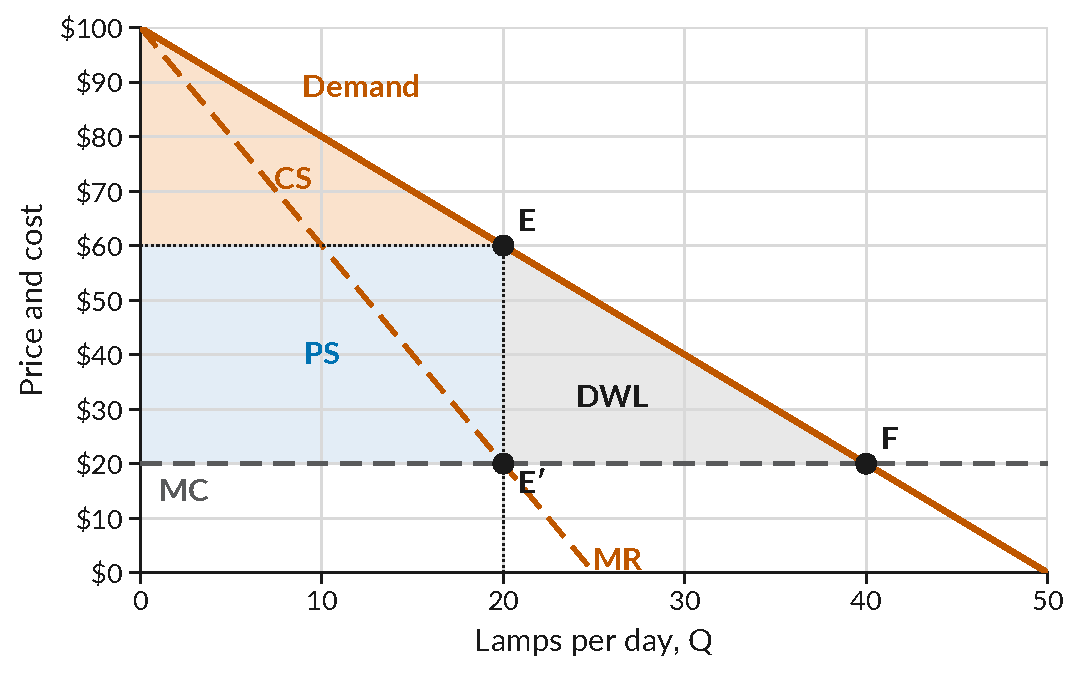
\includegraphics[width=0.47\linewidth, alt={Price and cost from 0 to 100
dollars on the vertical axis, lamps per day from 0 to 50 on the horizontal,
gridlines every 10. Demand falls in a straight line from 100 dollars at zero
lamps to zero at 50. A dashed marginal revenue line falls twice as steeply
from the same point. Marginal cost is a flat dashed line at 20 dollars. The
point E is on the demand curve at 20 lamps and 60 dollars, with dotted guides
to both axes; E prime is directly below it where marginal revenue meets
marginal cost; F is where demand meets marginal cost at 40 lamps. Consumer
surplus is the shaded triangle above 60 dollars out to 20 lamps, producer
surplus the shaded rectangle between 20 and 60 dollars out to 20 lamps, and
deadweight loss the shaded triangle between marginal cost and demand from 20
to 40 lamps.}]{figures/lamps.pdf}\par}


\step{Pareto Improvement.} The 30th buyer values a lamp at \$40, above its \$20 cost, so selling them one at \$30 leaves both \$10 better off and nobody worse off: $E$ is not Pareto efficient.

\step{Deadweight Loss.} Buyers 21 to 40 value a lamp above its \$20 cost but get none, since selling to them means a lower price for everyone. Demand meets MC at 40 lamps, the point $F$; the lost surplus is the triangle between demand and MC from 20 to 40 lamps: $\text{DWL} = \tfrac{1}{2} \times (40 - 20) \times (60 - 20) = 400$.



\newpage
\block{Your Turn}
Pine Desks' demand curve is $P = 60 - Q$, and each desk costs \$12 to make. It maximizes profit by selling 24 desks a week at \$36. The graph shows its demand curve and marginal cost.

\begin{center}
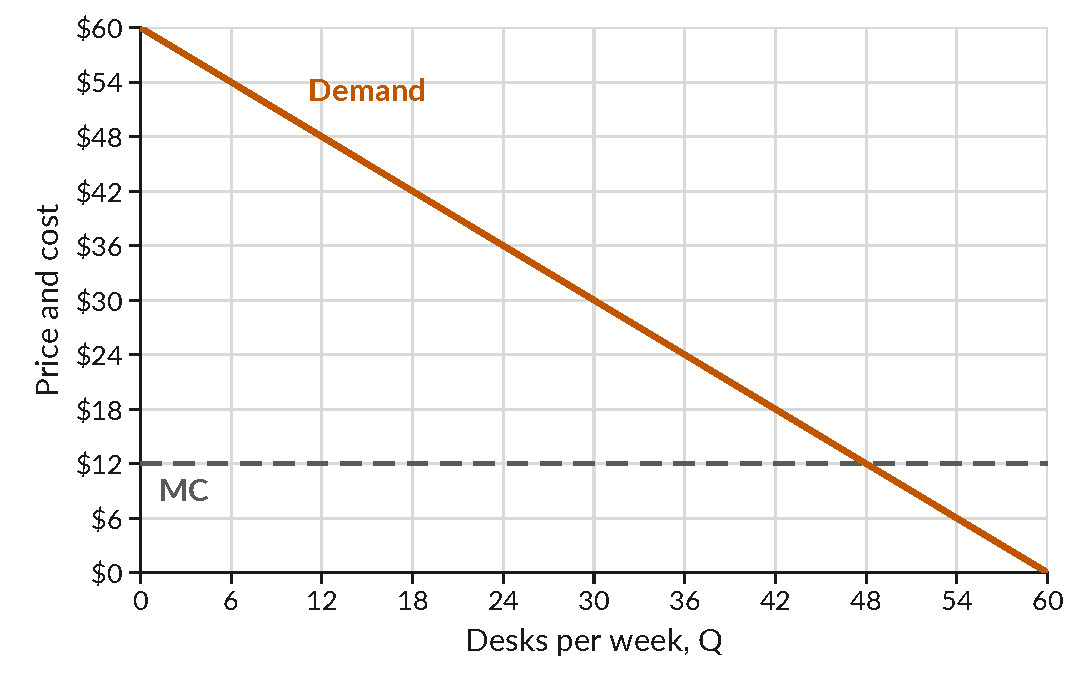
\includegraphics[width=0.5\linewidth, alt={A plotting grid, price and cost from 0 to 60 dollars on the vertical axis and desks per week from 0 to 60 on the horizontal, gridlines every 6. Demand falls in a straight line from 60 dollars at zero desks to zero at 60 desks. Marginal cost is a flat dashed line at 12 dollars. Nothing else is marked.}]{figures/desks.pdf}
\end{center}

(a) On the graph, draw a horizontal line at the price, \$36, and mark the profit-maximizing point $E$, 24 desks at \$36, on the demand curve. Then shade CS, PS, and DWL.

(b) The 12th buyer buys a desk at \$36. What are the buyer's gain, the firm's gain, and the joint surplus from that sale?

(c) Compute CS.

(d) Compute PS.

(e) Which buyers value a desk above its \$12 cost but do not buy at \$36? Give the range, from the \rule{1.2em}{0.4pt}th to the \rule{1.2em}{0.4pt}th buyer.

(f) Give a price at which selling a desk to the 36th buyer would be a Pareto improvement.

(g) Compute DWL.




% =====================================================================
\topicpage
\topic{Market Power and Competition}{Lectures 12 and 13}

\block{Can You? After Going Over the Slides, Check What Stuck}
\lec{Lecture 12}
\begin{itemize}
\cy{Say what market power is, and why a firm whose product has few close substitutes has it.}
\cy{Compute a firm's profit margin, $P - \text{MC}$, and its markup, $(P - \text{MC})/P$.}
\cy{State the markup rule, check whether a price follows it, and explain why less elastic demand means a higher markup.}
\cy{Name two sources of market power.}
\cy{Say what product differentiation is, how firms achieve it, and why it gives a firm market power.}
\cy{Explain why falling AC means only a few large firms survive.}
\cy{Say what a natural monopoly is.}
\cy{Name the four market structures and tell them apart by number of firms, products, entry, and control over price.}
\cy{Say what competition policy is for, and give the two ways firms limit competition.}
\end{itemize}
\lec{Lecture 13}
\begin{itemize}
\cy{Explain why, with only a few firms, one firm's best price depends on what its rivals charge.}
\cy{Explain why loyal customers keep prices high, and why buyers who compare prices drive them down.}
\cy{Explain why rivals who would all earn more charging high can still end up charging low, and why buyers gain from that.}
\end{itemize}

\block{Worked Example: A Roaster's Markup}
Bean There roasts coffee. Each bag costs it \$6 to make, it maximizes profit at \$10 a bag, and at that price the elasticity of its demand is $2.5$.

\step{Markup.} Profit margin $10 - 6 = \$4$ a bag. Markup $= (10 - 6)/10 = 0.4$: 40\% of the price is margin.

\step{The Markup Rule.} At the profit-maximizing price, $(P - \text{MC})/P = 1/\varepsilon$. Here $1/2.5 = 0.4$, the same as the markup, so the \$10 price follows the rule.

\step{A Rival Enters.} A second roaster opens and Bean There's buyers now have a close substitute, so its demand is more elastic: $\varepsilon = 5$. The rule gives a markup of $1/5 = 0.2$, so $(P - 6)/P = 0.2$, and $P = 7.50$. More substitutes, more elastic demand, lower markup, lower price.

\step{What If Rivals Are Few?} With many rivals, Bean There takes its demand curve as given. With one or two, its best price depends on what they charge: each would earn more if all charged high, but each gains by undercutting, so prices tend to end up low and buyers gain. The more loyal customers a firm has, the less this pressure bites.

\block{Your Turn}
Crust Bakery's loaves cost \$3 each to make. It maximizes profit at \$5 a loaf, where it sells 40 loaves a day, and every \$1 rise in price loses it 20 loaves.

(a) Find Crust's profit margin and markup.

(b) Find the price elasticity of demand at \$5.

(c) Does the \$5 price follow the markup rule?

(d) A second bakery opens nearby and the elasticity rises to 5. What price does the markup rule now give?

% =====================================================================
\topicpage
\pagestyle{plain}
\titlespacing*{\subsection}{0pt}{5pt}{0pt}
\section{Answers to Your Turn}\label{answers}
Check only after you have finished. For a part you got wrong, reread that step of the worked example.

\subsection{Opportunity Cost and Economic Rent}

(a) Net benefits 70 and 45. (b) Tutoring's net benefit, \$45. (c) Net benefit 70 $>$ 45, so she goes. (d) $50 + 45 = 95$; benefit 120 $>$ 95, the same decision. (e) $70 - 45 = 25$.

\subsection{Specialization and Comparative Advantage}

(a) Ava in cupcakes, Ben in pies. (b) Ava: a pie costs 4 cupcakes, a cupcake $\tfrac{1}{4}$ pie. Ben: 1 cupcake and 1 pie. (c) Ava in cupcakes, Ben in pies; each specializes there. (d) Yes: 2 cupcakes is above Ben's cost of a pie, 1 cupcake, and below Ava's, 4. (e) Between 1 and 4 cupcakes per pie.

\subsection{Costs, Demand, and the Profit-Maximizing Choice}

(a) $C(Q) = 96 + 6Q$. $\text{MC} = 6$ at every $Q$. $C(24) = 96 + 6 \times 24 = 240$, so $\text{AC} = 240/24 = 10$. Or, the fixed cost spread over 24 repairs plus MC: $96/24 + 6 = 4 + 6 = 10$.

(b) $\Delta Q / \Delta P = -2$: every \$1 rise loses 2 repairs. At $P = 0$, $Q = 60$. $2P = 60 - Q$, so $P = 30 - Q/2$, a line from $(0, 30)$ to $(60, 0)$.

(c) Price from $P = 30 - Q/2$, $R = P \times Q$, $C = 96 + 6Q$, profit $= R - C$:

\begin{center}
\vspace{2pt}
\begin{tabular}{@{}ZZZZZ@{}}
\toprule
$Q$ & $P$ & $R$ & $C(Q)$ & Profit \\
\midrule
20 & 20 & 400 & 216 & 184 \\
24 & 18 & 432 & 240 & 192 \\
28 & 16 & 448 & 264 & 184 \\
\bottomrule
\end{tabular}
\vspace{2pt}
\end{center}

(d) The 25th repair needs $P(25) = 30 - 25/2 = 17.50$, so $R(25) = 17.50 \times 25 = 437.50$ and $\text{MR} = R(25) - R(24) = 437.50 - 432 = 5.50$.

(e) The 25th repair adds \$5.50 to revenue, less than the \$6 MC, so going past 24 lowers profit; the 24th adds $432 - 425.50 = \$6.50$, more than MC, so it is worth doing. So $Q^* = 24$ and $P^* = 30 - 24/2 = \$18$, where the table's profit peaks at \$192.

(f) MR and MC are unchanged, so still 24 repairs at \$18. Profit falls by 30 at every quantity, to \$162.

(g) At its best price, 24 repairs bring in \$432 and cost $6 \times 24 = \$144$ in parts. That leaves $432 - 144 = \$288$ a day to pay the rent. If the rent were above \$288, the shop would lose money even at its best price, so it should not operate.

\subsection{Elasticity}

(a) 25\% and $-10\%$, so $\varepsilon = 0.4$, inelastic. (b) From the equation, $\Delta Q / \Delta P = -4$. At \$20, $Q = 120 - 4 \times 20 = 40$, so $\varepsilon = -\tfrac{P}{Q} \times \tfrac{\Delta Q}{\Delta P} = -\tfrac{20}{40} \times (-4) = 2$: elastic. (c) 20\% and 25\%, so 1.25: a normal good and a luxury. (d) $-20\%/20\% = -1$: complements.

\subsection{Surplus and Efficiency}

(a) The price line at \$36 meets the demand curve at $E$, $(24, 36)$; CS the triangle above \$36 out to 24, PS the rectangle between \$12 and \$36 out to 24, DWL between demand and MC from 24 to 48. (b) WTP $60 - 12 = \$48$; buyer's gain 12, firm's gain 24, joint surplus 36. (c) $\text{CS} = \tfrac{1}{2} \times 24 \times (60 - 36) = 288$. (d) $\text{PS} = (36 - 12) \times 24 = 576$. (e) The 25th to the 47th: their WTP, $60 - n$, is below \$36 and above \$12. (f) The 36th buyer's WTP is \$24, so any price between \$12 and \$24. (g) $\text{DWL} = \tfrac{1}{2} \times (48 - 24) \times (36 - 12) = 288$.

\subsection{Market Power and Competition}
(a) Margin $5 - 3 = \$2$; markup $2/5 = 0.4$. (b) $\varepsilon = \frac{5}{40} \times 20 = 2.5$. (c) Yes: $1/\varepsilon = 1/2.5 = 0.4$, the markup. (d) Markup $1/5 = 0.2$, so $(P - 3)/P = 0.2$ and $P = 3.75$.



\end{document}
